\def\year{2018}\relax
%File: formatting-instruction.tex
\documentclass[letterpaper]{article} %DO NOT CHANGE THIS
\usepackage{aaai18}  %Required
\usepackage{times}  %Required
\usepackage{helvet}  %Required
\usepackage{courier}  %Required
\usepackage{url}  %Required
\usepackage{graphicx}  %Required
\usepackage{mathtools}
\usepackage{amsmath}
\frenchspacing  %Required
\setlength{\pdfpagewidth}{8.5in}  %Required
\setlength{\pdfpageheight}{11in}  %Required
%PDF Info Is Required:
  \pdfinfo{
/Title (2018 Formatting Instructions for Authors Using LaTeX)
/Author (AAAI Press Staff)}
\setcounter{secnumdepth}{2}  
 \begin{document}
% The file aaai.sty is the style file for AAAI Press 
% proceedings, working notes, and technical reports.
%
\title{Unsupervised learning for joint depth and normal estimation}
\author{Zhenheng Yang \\
University of Southern California\\
\texttt{zhenheny@usc.edu}
\And 
Peng Wang\\
Baidu Research\\
\texttt{wangpeng54@baidu.com}
\And Ram Nevatia\\
University of Southern California\\
\texttt{nevatia@usc.edu}}

\maketitle
\begin{abstract}
We propose an unsupervised learning framework for joint estimation of scene depth and normal in single images. Similar to recent work [1,2,3], we implement an end-to-end network that leverages the view synthesis and geometry consistency in videos as the supervision. Our method takes monocular videos as input and outputs camera motion, depth and surface normal. Evaluation of depth and normal on KITTI 2015 dataset demonstrates the effectiveness of our approach: our method has outperforms current state-of-the-art performance in terms of depth and normal evaluation metrics.
\end{abstract}

\section{Introduction}

% introduce the problem
Depth and normal estimation has been explored in multiple 

\section{Related Work}

\subsection{Supervised depth and normal estimation}

\subsection{Unsupervised learning for low-level vision}

\subsection{Spatial transformer network}


\section{Method}
In this section, we describe the framework architecture and training procedure in detail.
Our intuition is to train a CNN that is capable of modeling the geometry consistency of a mostly rigid scene. To facilitate the learning of the network, we explicitly propose to model the constraint between depth and normal. The training samples of the framework consist of frame sequences captured by a monocular moving camera.
  
\subsection{Objective function}
To model a reasonable geometrical consistency, we propose the overall objective function as in Equation \ref{equ:1}.
\begin{equation}
\label{equ:1}
\begin{split}
L(D, I, Rt, \lambda) = L_{warp}(D, I, Rt) + L_{smooth}(D, N, I) \\
 +  L_{grad}(D, I, Rt) + \lambda(L_{dn}(D, N))
\end{split}
\end{equation}
This objective function is a Lagrange fuction aiming to minimize the loss term $L_{warp}(D, I, Rt) + L_{smooth}(D, N, I) \\
 +  L_{grad}(D, I, Rt)$ subject to the constraint of geometrical constraint between depth map and normal map $L_dn(D, N) = 0$. The loss term consists of three components: photometric warping loss $L_{warp}(D, I, Rt)$, smoothness loss $L_{smooth}(D, N, I)$, image gradient matching loss $L_{grad}(D, I, Rt)$.
 
\textbf{Photometric warping loss.} One main supervision of our framework comes from novel view synthesis: given an input view of a scene and camera motion, synthesize an image of the scene seen from a different view. We can synthesize an image of the target view given the image of source view, camera motion from target view to source view and depth map of target view, using 3D inverse warping. The process of warping is shown in Figure \ref{fig:3d_warping}.
\begin{figure}
\centering
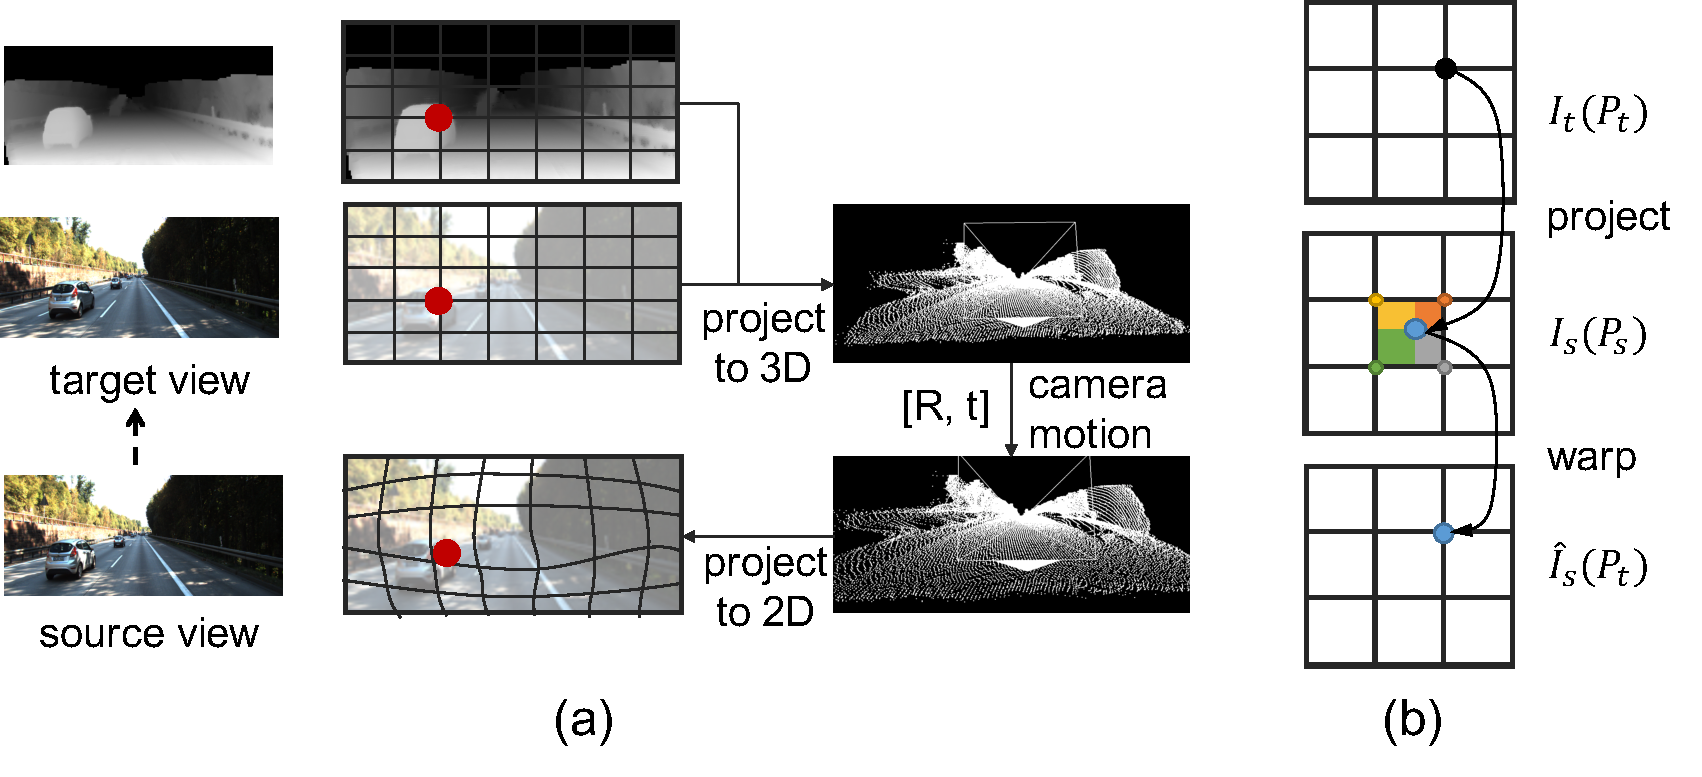
\includegraphics[width=0.5\textwidth]{figures/3d_warping.pdf}
\caption{Illustraion of (a) 3D inverse warping and (b) bilinear interpolation.}
\label{fig:3d_warping}
\end{figure}
Each pixel (point on the grid) of depth map is first mapped onto 3D space. The 3D point cloud is transformed based on camera motion and then mapped back to 2D plane. Each grid point in target view corresponds to one point in source view. Similar to \cite{jaderberg2015spatial}, the bilinear interpolation is implemented to calculate each pixel value of warped image as a weighted sum of four nearest neighboring pixels in source image, weighted by the square area between the projected point and neighboring point, as shown in Figure \ref{fig:3d_warping} (b).

The warping loss is a photometric difference between the target image and warped image. $$L_{warp}(D, I, Rt) = \sum_s\sum_p|I_t - \hat{I_s}|$$
In which, $s$ iterates the number of source image, $p$ iterates each pixel in the image, $I_t$ is the target image, $I_s$ is the source image, $\hat{I_s} = \tau(I_s, D_t, Rt)$ is the warped image, $\tau$ is the warping function as introduced above.

\textbf{Edge-aware smoothness loss.} One issue with using only view synthesis as supervision is that the back-propagation gradients are solely derived from the pixel value difference between one point in target image and weighted sum of its four neighboring points in source image. The warping loss will not be useful for learning where the point falls on low-texture regions. The predicted depth on these regions can be of any value as long as the warped region has the similar pixel value.  To overcome this issue, a prior knowledge of the scene geometry is incorporated for a smoothness loss:
\small
$$L_{smooth}(D) = \frac{1}{p} \sum_{p}(|\partial^2_xX_p|e^{(-\alpha||\partial_xI_p||)} + |\partial^2_yD_p|e^{(-\alpha||\partial_yI_p||)})$$
\normalsize

This smoothness term penalizes the norm of second-order gradients of depth in order to encourage smoothly changing depth values. As depth discontinuity often happens at image gradients, the smoothness loss is weighted by the a function of image gradients to prevent smoothed depth at image gradients. 

\textbf{Image gradient matching loss.}

To further facilitate the macthing of target image and warped image, and to encourage the depth map to be sharp, the photometric difference of gradient map of target image and gradient map of warped image is cacluated as image gradient matching loss.
$$L_{grad}(D, I, Rt) = \sum_s(|\partial_xI_t - \partial_x\hat{I}_s| + |\partial_yI_t - \partial_y\hat{I}_s|)$$


\subsection{Geometry consistency}

\textbf{Depth2normal layer.}

\textbf{Normal2depth layer.}

\section{Evaluation}

\subsection{Datasets and metrics}

\subsection{Ablation study}

\textbf{Depth and normal geometry consistency}

\textbf{Image edge in smoothness term}

\textbf{Image edge in depth2normal and normal2depth layers}

\textbf{Image gradient matching}

\subsection{Comparison with other methods}

\textbf{KITTI 2015 test split}

\textbf{KITTI 2015 Eigen split}

\section{Conclusion}

\noindent Congratulations on having a paper selected for inclusion in an AAAI Press proceedings or technical report! This document details the requirements necessary to get your accepted paper published using \LaTeX{}. If you are using Microsoft Word, instructions are provided in a different document. If you want to use some other formatting software, you must obtain permission from AAAI Press first. 

The instructions herein are provided as a general guide for experienced \LaTeX{} users. If you do not know how to use \LaTeX{}, do not use it to format your paper. AAAI cannot provide you with support and the accompanying style files are \textbf{not} guaranteed to work. If the results you obtain are not in accordance with the specifications you received, you must correct your source file to achieve the correct result. 

These instructions are generic. Consequently, they do not include specific dates, page charges, and so forth. Please consult your specific written conference instructions for details regarding your submission. Please review the entire document for specific instructions that might apply to your particular situation. All authors must comply with the following:

\begin{itemize}
\item You must use the 2018 AAAI Press \LaTeX{} style file and bib file, which are located in the 2018 author kit.
\item You must complete, sign, and return by the deadline the AAAI copyright form (proceedings authors) or distribution license (technical report authors).
\item You must read and format your paper source and PDF according to the formatting instructions for authors.
\item You must submit your electronic files and abstract using our electronic submission form \textbf{on time.}
\item You must pay any required page or formatting charges to AAAI Press so that they are received by the deadline.
\item You must check your paper before submitting it, ensuring that it compiles without error, and complies with the guidelines found in the author kit.
\end{itemize}

\section{Copyright}
All papers submitted for publication by AAAI Press must be accompanied by a valid signed copyright form or, in the case of technical reports, by a valid signed permission to distribute form. There are no exceptions to this requirement. You must send us the original version of this form. However, to meet the deadline, you may fax (1-650-321-4457) or scan and e-mail the form (pubforms18@aaai.org) to AAAI by the submission deadline, and then mail the original via postal mail to the AAAI office. \textbf{If you fail to send in a signed copyright or permission form, we will be unable to publish your paper. There are no exceptions to this policy.} You will find PDF versions of the AAAI copyright and permission to distribute forms in the author kit.

\section{Formatting Requirements in Brief}
We need source and PDF files that can be used in a variety of ways and can be output on a variety of devices. The design and appearance of the paper is governed by the aaai style file. 
\textbf{You must not make any changes to the aaai style file, nor use any commands, packages, style files, or macros within your own paper that alter that design, including, but not limited to spacing, floats, margins, fonts, font size, and appearance.} AAAI imposes  requirements on your source and PDF files that must be followed. Most of these requirements are based on our efforts to standardize conference manuscript properties and layout. All papers submitted to AAAI for publication will be recompiled for standardization purposes. Consequently, every paper submission must comply with the following requirements:

\begin{itemize}
\item Your .tex file must compile in PDF\LaTeX{} --- \textbf{ no .ps or .eps figure files.}
\item All fonts must be embedded in the PDF file --- \textbf{ this includes your figures.}
\item Modifications to the style file, whether directly or via commands in your document may not be made, most especially when made in an effort to avoid extra page charges or make your paper fit in a specific number of pages.
\item No type 3 fonts may be used (even in illustrations).
\item You may not alter the spacing above and below captions, figures, headings, and subheadings.
\item You may not alter the font sizes of text elements, footnotes, heading elements, captions, or title information (for references and tables and mathematics, please see the the limited exceptions provided herein).
\item You may not alter the line spacing of text.
\item Your title must follow Title Case capitalization rules (not sentence case).
\item Your .tex file must include completed metadata to pass-through to the PDF (see PDFINFO below)
\item \LaTeX{} documents must use the Times or Nimbus font package (do not use Computer Modern for the text of your paper).
\item No \LaTeX{} 209 documents may be used or submitted.
\item Your source must not require use of fonts for non-Roman alphabets within the text itself. If your paper includes symbols in other languages (such as, but not limited to, Arabic, Chinese, Hebrew, Japanese, Thai, Russian and other Cyrillic languages), you must restrict their use to bit-mapped figures.
\item Fonts that require non-English language support (CID and Identity-H) must be converted to outlines or 300 dpi bitmap or removed from the document (even if they are in a graphics file embedded in the document). 
\item Two-column format in AAAI style is required for all papers.
\item The paper size for final submission must be US letter without exception.
\item The source file must exactly match the PDF.
\item The document margins must be as specified in the formatting instructions.
\item The number of pages and the file size must be as specified for your event.
\item No document may be password protected.
\item Neither the PDFs nor the source may contain any embedded links or bookmarks.
\item Your source and PDF must not have any page numbers, footers, or headers.
\item Your PDF must be compatible with Acrobat 5 or higher.
\item Your \LaTeX{} source file (excluding references) must consist of a \textbf{single} file (use of the ``input" command is not allowed.
\item Your graphics must be sized appropriately outside of \LaTeX{} (do not use the ``clip" command) .
\end{itemize}

If you do not follow the above requirements, your submission will be subject to reformatting and special handling fees that can easily exceed the extra page fee.

\section{What Files to Submit}
You must submit the following items to ensure that your paper is published:
\begin{itemize}
\item A fully-compliant PDF file.
\item Your  \LaTeX{}  source file submitted as a \textbf{single} .tex file (do not use the ``input" command to include sections of your paper --- every section must be in the single source file). The only exception is the reference list, which you should include separately. Your source must compile on our system, which includes the standard \LaTeX{} support files.
\item Only the graphics files used in compiling paper.
\item The \LaTeX{}-generated files (e.g. .aux and .bib file, etc.) for your compiled source.
\item If you have used an old installation of \LaTeX{}, you should include algorithm style files). If in doubt, include it.
\end{itemize}

Your \LaTeX{} source will be reviewed and recompiled on our system (if it does not compile, you may incur late fees).   \textbf{Do not submit your source in multiple text files.} Your single \LaTeX{} source file must include all your text, your bibliography (formatted using aaai.bst), and any custom macros. Accompanying this source file, you must also supply any nonstandard (or older) referenced style files and all your referenced graphics files. 

Your files should work without any supporting files (other than the program itself) on any computer with a standard \LaTeX{} distribution. Place your PDF and source files in a single tar, zipped, gzipped, stuffed, or compressed archive. Name your source file with your last (family) name.

\textbf{Do not send files that are not actually used in the paper.} We don't want you to send us any files not needed for compiling your paper, including, for example, this instructions file, unused graphics files, standard style files, additional material sent for the purpose of the paper review, and so forth.

\textbf{Obsolete style files.}  The commands for some common packages (such as some used for algorithms), may have changed. Please be certain that you are not compiling your paper using old or obsolete style files. 

\section{Using \LaTeX{} to Format Your Paper}

The latest version of the AAAI style file is available on AAAI's website. Download this file and place it in  the \TeX\ search path. Placing it in the same directory as the paper should also work. You must download the latest version of the complete author kit so that you will have the latest instruction set and style file.

\subsection{Document Preamble}

In the \LaTeX{} source for your paper, you \textbf{must} place the following lines as shown in the example in this subsection. This command set-up is for three authors. Add or subtract author and address lines as necessary, and uncomment the portions that apply to you. In most instances, this is all you need to do to format your paper in the Times font. The helvet package will cause Helvetica to be used for sans serif. These files are part of the PSNFSS2e package, which is freely available from many Internet sites (and is often part of a standard installation).

Leave the setcounter for section number depth commented out and set at 0 unless you want to add section numbers to your paper. If you do add section numbers, you must uncomment this line and change the number to 1 (for section numbers), or 2 (for section and subsection numbers). The style file will not work properly with numbering of subsubsections, so do not use a number higher than 2.

If (and only if) your author title information will not fit within the specified  height allowed, put \textbackslash setlength \textbackslash titlebox{2.5in} in your preamble. Increase the height until the height error disappears from your log. You may not use the  \textbackslash setlength command elsewhere in your paper, and it may not be used to reduce the height of the author-title box.

\subsubsection{The Following Must Appear in Your Preamble}
\begin{quote}
\begin{scriptsize}\begin{verbatim}
\documentclass[letterpaper]{article}
\usepackage{aaai}
\usepackage{times}
\usepackage{helvet}
\usepackage{courier}
\usepackage{url}
\usepackage{graphicx}
\frenchspacing
% Add additional packages here. The following
% packages may NOT be used  (this list
% is not exhaustive:
% authblk, caption, CJK, float, fullpage, geometry, 
%hyperref, layout, nameref, natbib, savetrees, 
%setspace, titlesec, tocbibind, ulem
%
%US Lettersize Paper Is Required
\setlength{pdfpagewidth}{8.5in}
\setlength{pdfpageheight}{11in}\\
%
%
% PDFINFO
% You are required to complete the following
% for pass-through to the PDF. 
% No LaTeX commands of any kind may be
% entered. The parentheses and spaces 
% are an integral part of the 
% pdfinfo script and must not be removed.
%
\pdfinfo{
/Title (Input Your Paper Title Here)
/Author (John Doe, Jane Doe)
/Keywords (Input your keywords in this optional area)
}
%
%Section Numbers
% Uncomment if you want to use section numbers
% and change the 0 to a 1 or 2
% \setcounter{secnumdepth}{0}

% Title and Author Information Must Immediately Follow
% the pdfinfo within the preamble
%
\title{Title}\\
\author\{Author 1 \ and Author 2\\
Address line\\
Address line\\
\ And\\
Author 3\\
Address line\\
Address line
}\\
%
\end{verbatim}\end{scriptsize}
\end{quote}

\subsection{Preparing Your Paper}

After the preamble above, you should prepare your paper as follows:
\begin{quote}
\begin{scriptsize}\begin{verbatim}
%
\begin{document}
\maketitle
\begin{abstract}
%...
\end{abstract}\end{verbatim}\end{scriptsize}
\end{quote}

\subsubsection{The Following Must Conclude Your Document}
\begin{quote}
\begin{scriptsize}\begin{verbatim}
%References and End of Paper
%These lines must be placed at the end of your paper
\bibliography{Bibliography-File}
\bibliographystyle{aaai}
\end{document}
\end{verbatim}\end{scriptsize}
\end{quote}

\subsection{Inserting Document Metadata with \LaTeX{}}
PDF files contain document summary information that enables us to create an Acrobat index (pdx) file, and also allows search engines to locate and present your paper more accurately. \textit{Document metadata for author and title are REQUIRED.} You may not apply any script or macro to implementation of the title, author, and metadata information in your paper.

\textit{Important:} Do not include \textit{any} \LaTeX{} code or nonascii characters (including accented characters) in the metadata. The data in the metadata must be completely plain ascii. It may not include slashes, accents, linebreaks, unicode, or any \LaTeX{} commands. Type the title exactly as it appears on the paper (minus all formatting). Input the author names in the order in which they appear on the paper (minus all accents), separating each author by a comma. You may also include keywords in the Keywords field.




\begin{quote}
\begin{scriptsize}\begin{verbatim}
\begin{document}\\
\maketitle\\
...\\
\bibliography{Bibliography-File}\\
\bibliographystyle{aaai}\\
\end{document}\\
\end{verbatim}\end{scriptsize}
\end{quote}


\subsection{Illegal Commands}
There are a number of packages, commands, scripts, and macros that are incompatable with aaai18.sty. The common ones are provided later on in this document (See some Common  Errors to Avoid).  Generally, if a command, package, script, or macro alters floats, margins, fonts, sizing, linespacing, or the presentation of the references and citations, it is unacceptable. The following commands are some of the more common ones that may not be used in your paper (this list is not exhaustive --- there are others):
\begin{itemize}
\item \textbackslash renewcommand (in almost all instances)
\item \textbackslash baselinestretch
\item \textbackslash setlength (except for titlebox)
\item \textbackslash input
\item \textbackslash vspace or vskip (when used before or after a section or subsection or figure or table)
\item \textbackslash addtolength 
\item \textbackslash columnsep
\item \textbackslash top margin (or text height or addsidemargin or even side margin)
\item trim or clip (used to crop figures)
\item any command that globally alters floats, space above and below figures and tables
\end{itemize}

\subsection{Removing Certain Commands in Your Final Paper}
For your final camera ready copy, you must not use any page break commands, including, but not limited to:
\begin{itemize}
\item \textbackslash newpage
\item \textbackslash break
\item \textbackslash clearpage
\item \textbackslash pagebreak
\end{itemize}
(References must flow directly after the text without breaks.) Note that this may \textit{not} the case when submitting a paper for review. Some conferences require references to be on a separate page during the review process. AAAI Press, however, does not require this condition for the final paper. You must also be certain that your \textbackslash pdfino author field includes all your authors. The latter step is often forgotten.


\subsection{Paper Size, Margins, and Column Width}
Papers must be formatted to print in two-column format on 8.5 x 11 inch US letter-sized paper. The margins must be exactly as follows: 
\begin{itemize}
\item Top margin: .75 inches
\item Left margin: .75 inches
\item Right margin: .75 inches
\item Bottom margin: 1.25 inches
\end{itemize} 


The default paper size in most installations of \LaTeX{} is A4. However, because we require that your electronic paper be formatted in US letter size, the preamble we have provided includes commands that alter the default to US letter size. Please note that using any other package to alter page size (such as, but not limited to the Geometry package) will result in your final paper being rejected. 


\subsubsection{Column Width and Margins.}
To ensure maximum readability, your paper must include two columns. Each column should be 3.3 inches wide (slightly more than 3.25 inches), with a .375 inch (.952 cm) gutter of white space between the two columns. The aaai18.sty file will automatically create these columns for you. 

\subsection{Overlength Papers}
If your paper is too long, turn on \textbackslash frenchspacing, which will reduce the space after periods. Next,  shrink the size of your graphics. Use \textbackslash centering instead of \textbackslash begin\{center\} in your figure environment. For mathematical environments, you may reduce fontsize {\bf but not below 6.5 point}. You may also alter the size of your bibliography by inserting \textbackslash fontsize\{9.5pt\}\{10.5pt\} \textbackslash selectfont
right before the bibliography (the minimum size is \textbackslash fontsize\{9.0pt\}\{10.0pt\}. 

Commands that alter page layout are forbidden. These include \textbackslash columnsep, \textbackslash topmargin, \textbackslash topskip, \textbackslash textheight, \textbackslash textwidth, \textbackslash oddsidemargin, and \textbackslash evensizemargin (this list is not exhaustive). If you alter page layout, you will be required to pay the page fee \textit{plus} a reformatting fee. Other commands that are questionable and may cause your paper to be rejected include  \textbackslash parindent, and \textbackslash parskip. Commands that alter the space between sections are forbidden. The title sec package is not allowed. Regardless of the above, if your paper is obviously ``squeezed" it is not going to to be accepted. Options for reducing the length of a paper include reducing the size of your graphics, cutting text, or paying the extra page charge (if it is offered). 

\subsection{Figures}
Your paper must compile in PDF\LaTeX{}. Consequently, all your figures must be .jpg, .png, or .pdf. You may not use  the .gif (the resolution is too low), .ps, or .eps file format for your figures.

When you include your figures, you must crop them \textbf{outside} of \LaTeX{}. The command \textbackslash includegraphics*[clip=true, viewport 0 0 10 10]{...} might result in a PDF that looks great, but the image is \textbf{not really cropped.} The full image can reappear (and obscure whatever it is overlapping) when page numbers are applied or color space is standardized. 

\subsection{Type Font and Size}
Your paper must be formatted in Times Roman or Nimbus. We will not accept papers formatted using Computer Modern or Palatino or some other font as the text or heading typeface. Sans serif, when used, should be Courier. Use Symbol or Lucida or Computer Modern for \textit{mathematics only. } 

Do not use type 3 fonts for any portion of your paper, including graphics. Type 3 bitmapped fonts are designed for fixed resolution printers. Most print at 300 dpi even if the printer resolution is 1200 dpi or higher. They also often cause high resolution imagesetter devices and our PDF indexing software to crash. Consequently, AAAI will not accept electronic files containing obsolete type 3 fonts. Files containing those fonts (even in graphics) will be rejected. 

Fortunately, there are effective workarounds that will prevent your file from embedding type 3 bitmapped fonts. The easiest workaround is to use the required times, helvet, and courier packages with \LaTeX{}2e. (Note that papers formatted in this way will still use Computer Modern for the mathematics. To make the math look good, you'll either have to use Symbol or Lucida, or you will need to install type 1 Computer Modern fonts --- for more on these fonts, see the section ``Obtaining Type 1 Computer Modern.")

If you are unsure if your paper contains type 3 fonts, view the PDF in Acrobat Reader. The Properties/Fonts window will display the font name, font type, and encoding properties of all the fonts in the document. If you are unsure if your graphics contain type 3 fonts (and they are PostScript or encapsulated PostScript documents), create PDF versions of them, and consult the properties window in Acrobat Reader. 

The default size for your type should be ten-point with twelve-point leading (line spacing). Start all pages (except the first) directly under the top margin. (See the next section for instructions on formatting the title page.) Indent ten points when beginning a new paragraph, unless the paragraph begins directly below a heading or subheading.

\subsubsection{Obtaining Type 1 Computer Modern for \LaTeX{}.}

If you use Computer Modern for the mathematics in your paper (you cannot use it for the text) you may need to download type 1 Computer fonts. They are available without charge from the American Mathematical Society:
http://www.ams.org/tex/type1-fonts.html. 

\subsection{Title and Authors}
Your title must appear in mixed case (nouns, pronouns, and verbs are capitalized) near the top of the first page, centered over both columns in sixteen-point bold type (twenty-four point leading). This style is called ``mixed case." Author's names should appear below the title of the paper, centered in twelve-point type (with fifteen point leading), along with affiliation(s) and complete address(es) (including electronic mail address if available) in nine-point roman type (the twelve point leading). (If the title is long, or you have many authors, you may reduce the specified point sizes by up to two points.) You should begin the two-column format when you come to the abstract. 

\subsubsection{Formatting Author Information}
Author information can be set in a number of different styles, depending on the number of authors and the number of affiliations you need to display. In formatting your author information, however, you may not use a table nor may you employ the \textbackslash authorblk.sty package. For several authors from the same institution, use \textbackslash and:

\begin{quote}\begin{scriptsize}\begin{verbatim}
\author{Author 1 \and ... \and Author n\\ 
Address line \\ ... \\ Address line}
\end{verbatim}\end{scriptsize}\end{quote}

\noindent If the names do not fit well on one line use:

\begin{quote}\begin{scriptsize}\begin{verbatim}
\author{Author 1} ... \\
{\bf \Large Author  ...  Author}\\ 
Address line \\ ... \\ Address line
}
\end{verbatim}\end{scriptsize}\end{quote}

\noindent For authors from different institutions, use \textbackslash And:

\begin{quote}\begin{scriptsize}\begin{verbatim}
\author{Author 1\\ Address line \\ ... \\ Address line 
\And ... \And Author n\\
Address line\\ ... \\ Address line}
\end{verbatim}\end{scriptsize}\end{quote}

\noindent To start a separate ``row" of authors, use \textbackslash AND:

\noindent If the title and author information does not fit in the area allocated, place
\textbackslash setlength\textbackslash titlebox\{\textit{height}\}
after the \textbackslash documentclass line where \{\textit{height}\} is  2.5in or greater.

\subsubsection{Formatting Author Information --- Alternative Method}
If your paper has a large number of authors from different institutions, you may use the following alternative method for displaying the author information.

\begin{quote}\begin{scriptsize}\begin{verbatim}
\author{AuthorOne},\textsuperscript{1}
\author{AuthorTwo},\textsuperscript{2}
\author{AuthorThree},\textsuperscript{3}
\author{AuthorFour},\textsuperscript{4}
\author{AuthorFive}, \textsuperscript{5}\\
\textsuperscript{1}AffiliationOne}\\
\textsuperscript{2}AffiliationTwo}\\
\textsuperscript{3}AffiliationThree}\\
\textsuperscript{4}AffiliationFour}\\
\textsuperscript{5}AffiliationFive}\\
\{email, email\}@affiliation.com,
email@affiliation.com,
email@affiliation.com, 
email@affiliation.com
\end{verbatim}\end{scriptsize}\end{quote}


\subsection{\LaTeX{} Copyright Notice}
The copyright notice automatically appears if you use aaai.sty. If you are creating a technical report, it is not necessary to include this notice. You may disable the copyright line using the \verb+\+nocopyrightcommand. To change the entire text of the copyright slug, use:
\textbackslash copyrighttext \{\emph{text}\}.
Either of these must appear before \textbackslash maketitle. Please be advised, however, that \textit{if you disable or change the copyright line and transfer of copyright is required, your paper will not be published.}

\subsection{Credits}
Any credits to a sponsoring agency should appear in the acknowledgments section, unless the agency requires different placement. If it is necessary to include this information on the front page, use
\textbackslash thanks in either the \textbackslash author or \textbackslash title commands.
For example:
\begin{quote}
\begin{small}
\textbackslash title\{Very Important Results in AI\textbackslash thanks\{This work is
 supported by everybody.\}\}
\end{small}
\end{quote}
Multiple \textbackslash thanks commands can be given. Each will result in a separate footnote indication in the author or title with the corresponding text at the botton of the first column of the document. Note that the \textbackslash thanks command is fragile. You will need to use \textbackslash protect.

Please do not include \textbackslash pubnote commands in your document.

\subsection{Abstract}
Follow the example commands in this document for creation of your abstract. Further indentation is not required. {Do not include references in your abstract!}

\subsection{Page Numbers}

Do not \textbf{ever} print any page numbers on your paper. 

\subsection{Text }
The main body of the paper must be formatted in ten-point with twelve-point leading (line spacing).

\subsection{Citations}
Citations within the text should include the author's last name and year, for example (Newell 1980). Append lower-case letters to the year in cases of ambiguity. Multiple authors should be treated as follows: (Feigenbaum and Engelmore 1988) or (Ford, Hayes, and Glymour 1992). In the case of four or more authors, list only the first author, followed by et al. (Ford et al. 1997).

\subsection{Extracts}
Long quotations and extracts should be indented ten points from the left and right margins. 

\begin{quote}
This is an example of an extract or quotation. Note the indent on both sides. Quotation marks are not necessary if you offset the text in a block like this, and properly identify and cite the quotation in the text. 

\end{quote}

\subsection{Footnotes}
Avoid footnotes as much as possible; they interrupt the reading of the text. When essential, they should be consecutively numbered throughout with superscript Arabic numbers. Footnotes should appear at the bottom of the page, separated from the text by a blank line space and a thin, half-point rule. 

\subsection{Headings and Sections}
When necessary, headings should be used to separate major sections of your paper. Remember, you are writing a short paper, not a lengthy book! An overabundance of headings will tend to make your paper look more like an outline than a paper. The aaai.sty package will create headings for you. Do not alter their size nor their spacing above or below. 

\subsubsection{Section Numbers}
The use of section numbers in AAAI Press papers is optional. To use section numbers in \LaTeX{}, uncomment the setcounter line in your document preamble and change the 0 to a 1 or 2. Section numbers should not be used in short poster papers.

\subsubsection{Section Headings.}
Sections should be arranged and headed as follows: 

\subsubsection{Acknowledgments.}
The acknowledgments section, if included, appears after the main body of text and is headed ``Acknowledgments." This section includes acknowledgments of help from associates and colleagues, credits to sponsoring agencies, financial support, and permission to publish. Please acknowledge other contributors, grant support, and so forth, in this section. Do not put acknowledgments in a footnote on the first page. If your grant agency requires acknowledgment of the grant on page 1, limit the footnote to the required statement, and put the remaining acknowledgments at the back. Please try to limit acknowledgments to no more than three sentences. 

\subsubsection{Appendices.}
Any appendices follow the acknowledgments, if included, or after the main body of text if no acknowledgments appear. 

\subsubsection{References}
The references section should be labeled ``References" and should appear at the very end of the paper (don't end the paper with references, and then put a figure by itself on the last page). A sample list of references is given later on in these instructions. Please use a consistent format for references. Poorly prepared or sloppy references reflect badly on the quality of your paper and your research. Please prepare complete and accurate citations.

\subsection{Illustrations and Figures}
Figures, drawings, tables, and photographs should be placed throughout the paper near the place where they are first discussed. Do not group them together at the end of the paper. If placed at the top or bottom of the paper, illustrations may run across both columns. Figures must not invade the top, bottom, or side margin areas. Figures must be inserted using the \textbackslash usepackage\{graphicx\}. Number figures sequentially, for example, figure 1, and so on. 

The illustration number and caption should appear under the illustration. Labels, and other text with the actual illustration must be at least nine-point type. 

If your paper includes illustrations that are not compatible with PDF\TeX{} (such as .eps or .ps documents), you will need to convert them. The epstopdf package will usually work for eps files. You will need to convert your ps files to PDF however.



\subsubsection{Low-Resolution Bitmaps.}
You may not use low-resolution (such as 72 dpi) screen-dumps and GIF files---these files contain so few pixels that they are always blurry, and illegible when printed. If they are color, they will become an indecipherable mess when converted to black and white. This is always the case with gif files, which should never be used. The resolution of screen dumps can be increased by reducing the print size of the original file while retaining the same number of pixels. You can also enlarge files by manipulating them in software such as PhotoShop. Your figures should be 300 dpi when incorporated into your document.

\subsubsection{\LaTeX{} Overflow.}
\LaTeX{} users please beware: \LaTeX{} will sometimes put portions of the figure or table or an equation in the margin. If this happens, you need to scale the figure or table down, or reformat the equation.{ \bf Check your log file!} You must fix any overflow into the margin (that means no overfull boxes in \LaTeX{}). If you don't, the overflow text will simply be eliminated. \textbf{Nothing is permitted to intrude into the margin or gutter.}

\subsubsection{Using Color.}
Use of color is restricted to figures only. It may never be used for any portion of the text of your paper. The archival version of your paper will be printed in black and white and grayscale. Consequently, because conversion to grayscale can cause undesirable effects (red changes to black, yellow can disappear, and so forth), we strongly suggest you avoid placing color figures in your document. If you do include color figures, you must (1) use the CMYK (not RGB) colorspace and (2)  be mindful of readers who may happen to have a color deficiency. Your paper must be decipherable without using color for distinction. 

\subsubsection{Drawings.}
We suggest you use computer drawing software (such as Adobe Illustrator or, (if unavoidable), the drawing tools in Microsoft Word) to create your illustrations. Do not use Microsoft Publisher. These illustrations will look best if all line widths are uniform (half- to two-point in size), and you do not create labels over shaded areas. Shading should be 133 lines per inch if possible. Use Times Roman or Helvetica for all figure call-outs. \textbf{Do not use hairline width lines} --- be sure that the stroke width of all lines is at least .5 pt. Zero point lines will print on a laser printer, but will completely disappear on the high-resolution devices used by our printers.

\subsubsection{Photographs and Images.}
Photographs and other images should be in grayscale (color photographs will not reproduce well; for example, red tones will reproduce as black, yellow may turn to white, and so forth) and set to a minimum of 300 dpi. Do not prescreen images.

\subsubsection{Resizing Graphics.}
Resize your graphics \textbf{before} you include them with LaTeX. You may \textbf{not} use trim or clip options as part of your \textbackslash includegraphics command. Resize the media box of your PDF using a graphics program instead. 

\subsubsection{Fonts in Your Illustrations}
You must embed all fonts in your graphics before including them in your LaTeX document.

\subsection{References} 
The AAAI style includes a set of definitions for use in formatting references with BibTeX. These definitions make the bibliography style fairly close to the one specified below. To use these definitions, you also need the BibTeX style file ``aaai.bst," available in the author kit on the AAAI web site. Then, at the end of your paper but before \textbackslash end{document}, you need to put the following lines:

\begin{quote}
\begin{small}
\textbackslash bibliographystyle\{aaai\}
\textbackslash bibliography\{bibfile1,bibfile2,...\}
\end{small}
\end{quote}

Please note that you are required to use \textbackslash bibliographystyle\{aaai\} for your references. You may not use named, plain, apalike, acm, ieeetr, siam, chicago, or any other style. Use of natbib is also not acceptable.

The list of files in the \textbackslash  bibliography command should be the names of your BibTeX source files (that is, the .bib files referenced in your paper).

The following commands are available for your use in citing references:
\begin{quote}
\begin{small}
\textbackslash cite: Cites the given reference(s) with a full citation. This appears as ``(Author Year)'' for one reference, or ``(Author Year; Author Year)'' for multiple references.\\
\textbackslash shortcite: Cites the given reference(s) with just the year. This appears as ``(Year)'' for one reference, or ``(Year; Year)'' for multiple references.\\
\textbackslash citeauthor: Cites the given reference(s) with just the author name(s) and no parentheses.\\
\textbackslash citeyear: Cites the given reference(s) with just the date(s) and no parentheses.
\end{small}
\end{quote}

\textbf{Warning:} The aaai.sty file is incompatible with the hyperref and natbib packages. If you use either, your references will be garbled and your paper will not be published.

Formatted bibliographies should look like the following examples.

\smallskip \noindent \textit{Book with Multiple Authors}\\
Engelmore, R., and Morgan, A. eds. 1986. \textit{Blackboard Systems.} Reading, Mass.: Addison-Wesley.

\smallskip \noindent \textit{Journal Article}\\
Robinson, A. L. 1980a. New Ways to Make Microcircuits Smaller. \textit{Science} 208: 1019--1026.

\smallskip \noindent \textit{Magazine Article}\\
Hasling, D. W.; Clancey, W. J.; and Rennels, G. R. 1983. Strategic Explanations in Consultation. \textit{The International Journal of Man-Machine Studies} 20(1): 3--19.

\smallskip \noindent \textit{Proceedings Paper Published by a Society}\\
Clancey, W. J. 1983. Communication, Simulation, and Intelligent Agents: Implications of Personal Intelligent Machines for Medical Education. In \textit{Proceedings of the Eighth International Joint Conference on Artificial Intelligence,} 556--560. Menlo Park, Calif.: International Joint Conferences on Artificial Intelligence, Inc.

\smallskip \noindent \textit{Proceedings Paper Published by a Press or Publisher}\\
Clancey, W. J. 1984. Classification Problem Solving. In \textit{Proceedings of the Fourth National Conference on Artificial Intelligence,} 49--54. Menlo Park, Calif.: AAAI Press. 

\smallskip \noindent \textit{University Technical Report}\\
Rice, J. 1986. Poligon: A System for Parallel Problem Solving, Technical Report, KSL-86-19, Dept. of Computer Science, Stanford Univ. 

\smallskip \noindent \textit{Dissertation or Thesis}\\
Clancey, W. J. 1979. Transfer of Rule-Based Expertise through a Tutorial Dialogue. Ph.D. diss., Dept. of Computer Science, Stanford Univ., Stanford, Calif.

\smallskip \noindent \textit{Forthcoming Publication}\\
Clancey, W. J. 1986. The Engineering of Qualitative Models. Forthcoming.


\section{Some Common Errors to Avoid}

The following list includes a number of the most common mistakes made by authors when formatting their paper and the reponses that have been sent to the author regarding them:

\begin{small}
\begin{quote}
PDFINFO\\
The following required elements are missing from the preamble to your LaTeX source (or are malformed):
\begin{small}\begin{verbatim}
\pdfinfo{ 
/Title () 
/Author () 
}
\end{verbatim}\end{small}



A4\\
The PDF you submitted is A4. All PDFs must be US Letter sized. Submissions that do not conform to this requirement cannot be published. 
\smallskip


ABOVEDISPLAY\\
You've used \textbackslash abovedisplay, \textbackslash belowdisplay, \textbackslash above caption, and \textbackslash belowcaption to alter aaai18.sty. These commands are illegal and must be stripped from your source.
\smallskip


ABSTRACT INDENTATION\\
Remove the \textbackslash begin\{quote\} and \textbackslash \{endquote\} around your abstract. It might buy you some space.
\smallskip


ASPECT RATIO OF FIGURES CHANGED\\
You may scale the height OR the width of your figures, but not both.
\smallskip


AUTHOR LIST MALFORMED (AUTHBLK)\\
The authblk.sty package cannot be used. 
\smallskip


AUTHOR LIST MALFORMED\\
You did not use the built-in commands in aaai18.sty to format your authors. You need to follow the formatting instructions for authors using LaTeX. 
\smallskip


AUTHOR LIST TOO WIDE\\
Your author list goes beyond the accepted page width. Please break the line and insert \{\textbackslash bf \textbackslash Large\} around the authors on the second line. The author and title information must be presented as specified in the author instructions.
\smallskip


AUTHOR AFFLIATIONS TOO WIDE\\
Your author's affiliations go beyond the accepted page width. Please break the line.
\smallskip


BASELINESTRETCH\\
You've used \textbackslash baselinestretch --- a command specifically prohibited in the author formatting instructions. Please remove it.
\smallskip


CAPTION STYLE ALTERED (CAPTION.STY)\\
You've altered the font and style of captions. Captions must be rendered as specified by aaai.sty. They cannot be altered by changing the font, fontsize, or position, whether manually or by using caption.sty. Such revisions must be removed.
\smallskip


CJK\\
The CJK package cannot be used. Restrict use of non-roman alphabets to figures and tables, which must be compiled and converted to PDF, then imported as a figure into LaTeX.
\smallskip


CLIP\\
You may not use the clip to import only a portion of a graphic. It only places a fragile layer that screens the remained of the figure from view, but imports the entire figure into the PDF. The layer is fragile, and often fails when flattened. The full content of all figures must be imported. In addition and for the same reason, you may not use vspace to reposition a figure. All figures must be completely cropped and adjusted outside of LaTeX before being imported. 
\smallskip


COLUMN WIDTH\\
Unfortunately, your paper contains material that exceeds the column width. Please review your LaTeX log file and correct all the overfull boxes.
\smallskip


COMPILE ERRORS\\
Unfortunately, the source file you submitted will not compile. We are getting undefined control sequence errors. There are either missing packages in your preamble, or missing definitions, or perhaps you are using an old or modified style. For your information, we are using a complete 2017 install of TeXLive, complete with all updates as of September 1. The packages listed in your preamble are all installed on all our systems. If you are using a style file that is not in that package, you will need to include it. Whatever the reason, we need you to correct your LaTeX and resubmit your source files. (If your paper contains graphics, be certain that the fonts are embedded.) 
\smallskip


EPSF / EPSFIG / PSFIG\\
The epsf, epsfig, and psfig packages are obsolete. Use the graphicx package instead.
\smallskip


EULER\\
The euler package is obsolte
\smallskip


FIGURES HAVE BEEN CROPPED WITH LATEX\\
You have used trim and clip commands in your \textbackslash includegraphics statement. Please crop your graphics appropriately using a standard graphics program (not Preview). The masks created by LaTeX are fragile, and disappear when PDFs are combined together. This will result in text in your paper becoming obscured by the fully restored graphic you have imported.
\smallskip


FIGURES MISSING\\
Unfortunately, the source file you submitted are incomplete. You did not include the graphics files. As a result, your paper will not compile. You must upload a new compressed archive that contains all the files required to compile your paper on a different computer and network. (If your paper contains graphics, be certain that the fonts are embedded.) 
\smallskip

FLOATS ALTERED\\
You've altered floats.  The \textbackslash renewcommand cannot be used. The float package cannot be used. Please remove them.
\smallskip


FOOTNOTE STYLE ALTERED\\
Footnotes must follow the built-in style.
\smallskip


FONTS (EMBEDDING)\\
Unfortunately, one or more of the fonts in your paper (most likely the figures) were not embedded in your PDF. This can cause hidden and silent changes to characters once the paper is published, especially when it is combined with other PDFs in the proceedings. If you need to know how to verify the fonts in your figures, please search for ``font embedding pdf." You will find a number of methods, one or more of which may be suitable for your operating system and available software. We recommend using Acrobat Reader to check document properties in your PDF, as it is standards-based software. Consequently, you must embed all the fonts in all your graphics files. If you do not know how to do this, change them to png or jpg. 
\smallskip


FONTS (LANGUAGE)\\
We cannot accept files that require custom installation of non-roman font sets, including CJK and arabic.
 \smallskip


FONTS (TYPE 3)\\
Unfortunately, one or more of the fonts in your paper (most likely the figures) are type 3 PDF. If in your figures, you must either change them to type 1 embedded fonts or change them to png or jpg. If the problem is in your text, you will need to switch the package you are using that is calling type 3 fonts to one that uses type 1 fonts. (Blackboard fonts are often the problem in these cases.)
\smallskip


FULL PAGE USED\\
You used \textbackslash usepackage\{full page\}, which is a package specifically disallowed. You must remove it.
\smallskip


GEOMETRY USED\\
You used \textbackslash usepackage\{geometry\}, which is a package specifically disallowed. You must remove it.
\smallskip


GRAPHICS\\
The graphics package is obsolete. Use the graphicx package instead.
\smallskip


HYPERREF\\
The hyperref package may never be used. If you are using it for URLs, use url.sty instead
\smallskip


INCOMPATIBLE SCRIPT OR MACRO\\
You've used an incompatible script (such as \textbackslash maltepaper.sty) to automate completion of the title and author information on your paper and in the metadata. Such scripts impede correction of your paper and often are incompatible with Acrobat (producing corrupted metadata fields). Scripts and macros cannot be used to automate population of metadata, author or title information, or insertion of figures or tables.
\smallskip


LAYOUT\\
The layout package cannot be used. Use url.sty instead.
\smallskip


LINESPREAD\\
\textbackslash linespread alters aaai.sty. This command (along with \textbackslash baselineshift and others that alter aaai.sty) cannot be used. You must remove it.
\smallskip


LMODERN\\
You used \textbackslash usepackage\{lmodern\}, which is a package specifically disallowed. You must remove it.
\smallskip


LAYOUT USED\\
You used \textbackslash usepackage\{layout\}, which is a package specifically disallowed. You must remove it.
\smallskip


MBOX USED FOR FIGURES\\
You cannot use mboxes to insert figures. They circumvent the spacing requirements for aaai.sty. Use subfigures instead.
\smallskip


MULTIPLE TEX FILES\\
You did not submit a single .tex file as specified in the instructions. We require this to avoid production errors and to facilitate debugging. The \textbackslash input command is not allowed in your source. Please combine all your tex files into a single .tex file (references can remain in .bbl or .bib file).
\smallskip


NAMEREF\\
The nameref package cannot be used.
\smallskip


NATBIB\\
Natbib is incompatible with aaai18.sty and aaai.bst. It must be removed. See References Malformed below.
\smallskip
\smallskip


PAGE BREAKS \\
You've included pagebreaks in your final submission. (They are not required before your references accepted final papers and must be removed).
\smallskip

PAGE NUMBERS\\
Your paper contains page numbers. You need to remove them.
\smallskip

PDFLaTeX NOT USED\\
Your source will not compile in PDFLaTeX. You must convert your eps graphics to PDF.
\smallskip


PDFCOMMENT\\
You used pdfcomment, which is a disallowed package. You must remove it.
\smallskip


PSTRICKS\\
You used pstricks, which is a package specifically disallowed. You must remove it. (Use Tikz instead). If you are simply adding labels, use pinlabel.sty.
\smallskip


REFERENCES ARE INDENTED\\
You've indented your references. Remove the \textbackslash begin\{quote\} and \textbackslash end{quote}
\smallskip


REFERENCES MALFORMED\\
You've used natbib, which is incompatible with aaai.bst.

As an alternate to this, try this workaround:

\begin{quote}\begin{scriptsize}\begin{verbatim}% \usepackage{natbib}
\newcommand{\citet}[1]
{\citeauthor{#1}~\shortcite{#1}}
\newcommand{\citep}{\cite}
\newcommand{\citealp}[1]
{\citeauthor{#1}~\citeyear{#1}}\end{verbatim}\end{scriptsize}\end{quote}
\smallskip


REFERENCES TOO SMALL\\
Your references are too small. They cannot be any smaller than 9 pt (\textbackslash small). Please correct this.
 \smallskip


SAVETREES\\
The savetrees may not be used.
\smallskip


SETLENGTH\\
You've used \textbackslash setlength to alter textfloats. This command is specifically disallowed. Please strip it from your source and recompile.
\smallskip


SETSPACE\\
The setspace package may not be used.
\smallskip


SPACE ABOVE, BELOW ELEMENTS ALTERED\\
You've adjusted the space above or below tables, figures, captions, floats, and/or section/subsection/subsubsections. These changes alter aaai.sty and are not allowed. Please remove them and either edit your text or resize figures or both.
\smallskip


SOURCE FILES MISSING\\
Your compressed archive does not contain *ALL* your source files (a stand-alone archive containing all the files necessary to recompile your paper in LaTeX). Consequently, your LaTeX file will not compile. You must create another compressed archive in which you have included all the files necessary to compile your paper on a separate computer. We cannot publish your paper without these files.
\smallskip


SPACE ALTERED ABOVE, BELOW FLOATS AND SECTIONS\\
You've adjusted the space above or below tables, figures, captions, and/or section/subsection/subsubsections. These changes alter aaai.sty and have resulted in a paper that is more difficult to read. Please remove them and either edit your text or resize figures or both.
\smallskip


STYLE FILE OF BIBLIOGRAPHY IS INCORRECT\\
You did not use aaai.bst (you used named.bst instead). This is not an IJCAI conference. You need to recompile your bibliography using the correct style for AAAI-18.
\smallskip


STYLE FILE IS INCORRECT\\
You did not use aaai18.sty. This style file is required. No other style file (including previous versions of aaai.sty) may be used.
\smallskip


STYLE FILE NOT IN CTAN\\
All styles must be available in the CTAN archive. If they are custom, you need to remove them and put the contents of the custom style directly in your preamble so that our source checker will allow compilation of your file.
\smallskip


TIMES PACKAGE NOT USED\\
Your paper is not formatted using the Times package, either because it is missing completely from your preamble, or because you are using another package that is cancelling use of times. This package is required.
\smallskip


TITLESEC\\
The title sec package may not be used.
\smallskip


VSPACE USED\\
You've used negative vspace around section / subsections. These must be removed.
\smallskip


TIMES PACKAGE MISSING\\
You neglected to use \textbackslash usepackage\{times\}. This font is required.
\smallskip


TITLE AND AUTHOR INFORMATION MALFORMED\\
You need to remove the formatting commands from your title and author information. The style for this information is governed by the conference style file. It cannot be altered.
\smallskip


TITLE BOX TOO SMALL\\
Your author-title-affiliation data exceeds the limit of the title box. To
fix this, you need to increase the size of the title box. You can do this by
placing
\textbackslash setlength\textbackslash titlebox\{2.5in\} in your preamble. You may need to increase the measurement until
the log file error goes away. (Please note: This command cannot be used elsewhere
in the paper, and cannot be used to shrink the size of the title box.)
\smallskip


TITLE IN SENTENCE CASE\\
Your title is formatted in sentence case. Title Case (Mixed Case) is required. Please capitalize the initial letters of all words in your title except for conjunctions and prepositions. You need to do this in your source, in the \textbackslash pdfinfo in your source, and on the submission website.
\smallskip


TITLE MALFORMED (TITLESEC)\\
You've used titlesec.sty, which alters the AAAI style. It must be removed.
\smallskip


TOCBIBIND\\
The tocbibind package may not be used.
\smallskip


ULEM\\
The ulem package may not be used.
\smallskip


T1ENC\\
The T1enc package is obsolete. Us the CM Super Fonts package instead.



\end{quote}
\end{small}


\section{Producing Reliable PDF\\Documents with \LaTeX{}}
Generally speaking, PDF files are platform independent and accessible to everyone. When creating a paper for a proceedings or publication in which many PDF documents must be merged and then printed on high-resolution PostScript RIPs, several requirements must be met that are not normally of concern. Thus to ensure that your paper will look like it does when printed on your own machine, you must take several precautions:
\begin{itemize}
\item Use type 1 fonts (not type 3 fonts)
\item Use only standard Times, Nimbus, and CMR font packages (not fonts like F3 or fonts with tildes in the names or fonts---other than Computer Modern---that are created for specific point sizes, like Times\~{}19) or fonts with strange combinations of numbers and letters
\item Embed all fonts when producing the PDF
\item Do not use the [T1]{fontenc} package (install the CM super fonts package instead)
\end{itemize}

\subsection{Creating Output Using PDF\LaTeX{} Is Required}
By using the PDF\TeX{} program instead of straight \LaTeX{} or \TeX{}, you will probably avoid the type 3 font problem altogether (unless you use a package that calls for metafont). PDF\LaTeX{} enables you to create a PDF document directly from \LaTeX{} source. The one requirement of this software is that all your graphics and images must be available in a format that PDF\LaTeX{} understands (normally PDF, jpg, or png).

PDF\LaTeX{}'s default is to create documents with type 1 fonts. If you find that it is not doing so in your case, it is likely that one or more fonts are missing from your system or are not in a path that is known to PDF\LaTeX{}.

\subsubsection{dvipdf Script}
Scripts such as dvipdf which ostensibly bypass the Postscript intermediary should not be used since they generally do not instruct dvips to use the config.pdf file.

\subsubsection{dvipdfm}
Do not use this dvi-PDF conversion package.

\subsection{Ghostscript}
\LaTeX{} users should not use GhostScript to create their PDFs.

\subsection{Graphics}
If you are still finding type 3 fonts in your PDF file, look at your graphics! \LaTeX{} users should check all their imported graphics files as well for font problems.

\section{Proofreading Your PDF}
Please check all the pages of your PDF file. Is the page size A4? Are there any type 3, Identity-H, or CID fonts? Are all the fonts embedded? Are there any areas where equations or figures run into the margins? Did you include all your figures? Did you follow mixed case capitalization rules for your title? Did you include a copyright notice? Do any of the pages scroll slowly (because the graphics draw slowly on the page)? Are URLs underlined and in color? You will need to fix these common errors before submitting your file. 

\section{Improperly Formatted Files }
In the past, AAAI has corrected improperly formatted files submitted by the authors. Unfortunately, this has become an increasingly burdensome expense that we can no longer absorb. Consequently, if your file is improperly formatted, it will not be included in the publication. If time allows, however, you will be notified via e-mail of the problems with your file and given the option of correcting the file yourself. A resubmission fee (minimum \$50.00, and likely higher) will be required for this service). Optionally, you may ask that AAAI have the file corrected for you, for an additional fee. If you opt to correct the file yourself, please note that we cannot provide you with any additional advice beyond that given in your packet. Files that are not corrected after a second attempt will not be included in the publication.

\subsection{\LaTeX{} 209 Warning}
If you use \LaTeX{} 209 we will not be able to publish your paper. Convert your paper to \LaTeX{}2e.

\section{Naming Your Electronic File}
We request that you name your \LaTeX{} source file with your last name (family name) so that it can easily be differentiated from other submissions. If you name your files with the name of the event or ``aaai" or ``paper" or ``camera-ready" or some other generic or indecipherable name, you bear all risks of loss --- it is extremely likely that your file may be overwritten.

\section{Submitting Your Electronic Files to AAAI}
Submitting your files to AAAI is a two-step process. It is explained fully in the author registration and submission instructions. Please consult this document for details on how to submit your paper.

\section{Inquiries} 
If you have any questions about the preparation or submission of your paper as instructed in this document, please contact AAAI Press at the address given below. If you have technical questions about implementation of the aaai style file, please contact an expert at your site. We do not provide technical support for \LaTeX{} or any other software package. To avoid problems, please keep your paper simple, and do not incorporate complicated macros and style files.

\begin{quote}
\noindent AAAI Press\\
2275 East Bayshore Road, Suite 160\\
Palo Alto, California 94303\\ 
\textit{Telephone:} (650) 328-3123\\ 
\textit{E-mail:} See the submission instructions for your particular conference or event.
\end{quote}

\section{Additional Resources}
\LaTeX{} is a difficult program to master. If you've used that software, and this document didn't help or some items were not explained clearly, we recommend you read Michael Shell's excellent document (testflow doc.txt V1.0a 2002/08/13) about obtaining correct PS/PDF output on \LaTeX{} systems. (It was written for another purpose, but it has general application as well). It is available at www.ctan.org in the tex-archive.

\section{ Acknowledgments}
AAAI is especially grateful to Peter Patel Schneider for his work in implementing the aaai.sty file, liberally using the ideas of other style hackers, including Barbara Beeton. We also acknowledge with thanks the work of George Ferguson for his guide to using the style and BibTeX files --- which has been incorporated into this document  --- and Hans Guesgen, who provided several timely modifications, as well as the many others who have, from time to time, sent in suggestions on improvements to the AAAI style. 

The preparation of the \LaTeX{} and Bib\TeX{} files that implement these instructions was supported by Schlumberger Palo Alto Research, AT\&T Bell Laboratories, Morgan Kaufmann Publishers, The Live Oak Press, LLC, and AAAI Press. Bibliography style changes were added by Sunil Issar. \verb+\+pubnote was added by J. Scott Penberthy. George Ferguson added support for printing the AAAI copyright slug. Additional changes to aaai.sty and aaai.bst have been made by the AAAI staff.

\bigskip
\noindent Thank you for reading these instructions carefully. We look forward to receiving your electronic files!
\bibliographystyle{aaai.bst}
\bibliography{formatting-instructions-latex-2018.bib}
\end{document}
